% A first local projection on data: real GDP relative to potential on
% Ramey-Zubairy military news, controlling only for y_{t-1}, h = 0..20
% quarters. Point estimates only; no bands until Lectures 5 and 6.
\documentclass[border=3pt]{standalone}
% ————— Shared preamble for the course figures —————
% Each figure is a standalone TikZ document. build.sh compiles it to a PDF (for
% the LaTeX build) and converts that to an SVG (for the web build).
%
% Nothing is drawn in pure black: the chrome sits at a mid grey that stays
% legible on white paper and on the site's dark theme alike. Data colours are
% the course palette, the same blue and orange used in the practicum.

\usepackage{amsmath}
\usepackage{tikz}
\usepackage{pgfplots}
\pgfplotsset{compat=1.18}
\usepgfplotslibrary{fillbetween,groupplots}
\usetikzlibrary{arrows.meta,positioning,calc,backgrounds}

\definecolor{nwBlue}{HTML}{2A78D6}
\definecolor{nwOrange}{HTML}{D9601F}
\definecolor{nwMut}{HTML}{898781}
\definecolor{nwInk}{HTML}{6B6965}

\pgfplotsset{
  nwaxis/.style={
    axis lines=left,
    axis line style={nwMut, line width=0.5pt},
    tick align=outside,
    tick style={nwMut, line width=0.5pt},
    label style={text=nwInk, font=\small},
    tick label style={text=nwMut, font=\footnotesize},
    legend cell align=left,
    legend style={draw=none, fill=none, font=\footnotesize, text=nwInk,
                  row sep=1pt, inner sep=1pt},
    every axis plot post/.append style={line join=round},
    clip mode=individual,
  },
}

\directlua{dofile("fig-l01-first-contact-data.lua")}
\begin{document}
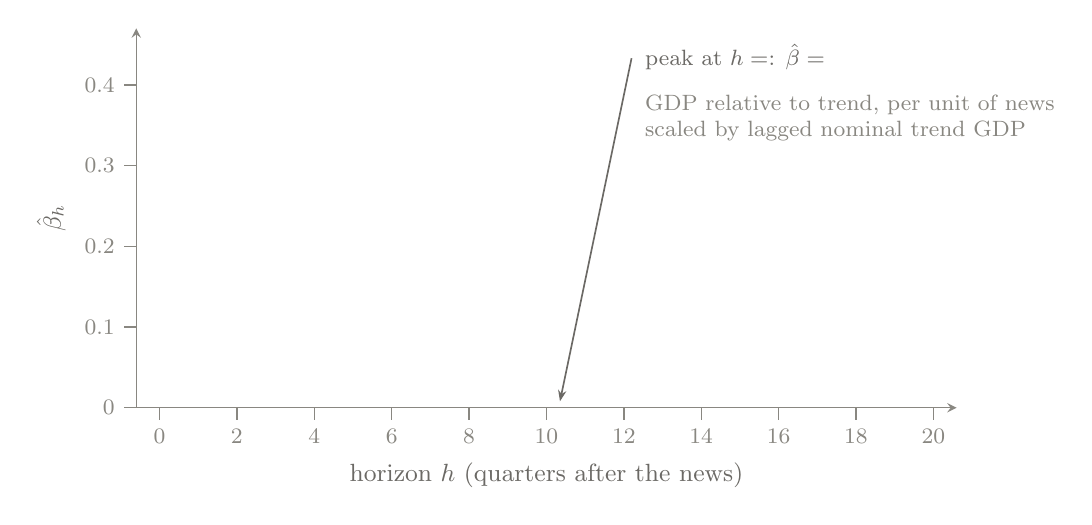
\begin{tikzpicture}
\begin{axis}[
  nwaxis,
  width=12cm, height=6.4cm,
  xmin=-0.6, xmax=20.6, ymin=0, ymax=0.47,
  xtick={0,2,...,20},
  ytick={0,0.1,0.2,0.3,0.4},
  yticklabels={$0$,$0.1$,$0.2$,$0.3$,$0.4$},
  xlabel={horizon $h$ (quarters after the news)},
  ylabel={$\hat\beta_h$},
]

\addplot[nwBlue, line width=1.3pt, mark=*, mark size=1.6pt,
         mark options={fill=nwBlue, draw=nwBlue}] coordinates {\lpFcBhat};

\node[text=nwInk, font=\footnotesize, anchor=west]
  at (axis cs:12.3,0.435) {peak at $h=\lpFcPeakH$: $\hat\beta_{\lpFcPeakH}=\lpFcPeakLab$};
\draw[nwInk, line width=0.6pt, -{Stealth[length=4pt,width=3pt]}]
  (axis cs:12.2,0.433) -- (axis cs:10.35,\lpFcPeakB+0.008);

\node[text=nwMut, font=\footnotesize, anchor=north west, align=left]
  at (axis cs:12.3,0.40)
  {GDP relative to trend, per unit of news\\
   scaled by lagged nominal trend GDP};

\end{axis}
\end{tikzpicture}
\end{document}
